\section{Task 2} \label{sec:Task2}

Für die Auslegung des Filters wurden die theoretischen Werte der benötigten Bauelemente berechnet, um die Cutoff-Frequenz optimal anzupassen und unerwünschte Störungen zu reduzieren. Ein Filterdesign, das in der Vorlesung besprochen wurde, wurde verwendet, um Resonanzspitzen zu unterdrücken. Eine zusätzliche Dämpfungsstruktur (Damping Branch) wurde integriert, um die Effektivität des Filters weiter zu steigern.

Die Schaltung in abbildung \ref{fig:LTC3639MitFilter} wurde um diesen Filter erweitert, um die EMV-Richtlinien einzuhalten und die leitungsgebundenen Emissionen sowohl im Common-Mode- als auch im Differential-Mode-Bereich zu reduzieren. Abbildung 2 zeigt die erweiterte Schaltung mit dem implementierten Filter, das zur Verbesserung der elektromagnetischen Verträglichkeit beiträgt.

Aufgaben und Auswahl der Komponenten:

\begin{itemize}
    \item \( C_f \) wirkt auf hohe Frequenzen und muss daher ein hochwertiger Kondensator sein, idealerweise ein Keramikkondensator.
    \item \( D_c \) beeinflusst niedrige Frequenzen und kann ein günstiger Elektrolytkondensator sein.
    \item \( C_d \) ist etwa 10- bis 20-mal größer als \( C_f \), um eine effektive Filterwirkung zu gewährleisten.
\end{itemize}

Dieses Design sorgt für eine effektive Dämpfung sowohl von differenziellen als auch von Gleichtaktstörungen und trägt dazu bei, die EMV-Anforderungen zu erfüllen. 

1. Induktivität \(L_f\):
\begin{equation}
    L_f = \frac{\left(\frac{1}{f_g \cdot 2 \pi}\right)^2}{C_f}
    \label{eqn:EffektiveKonvergenzordnung}
\end{equation} 

2. Charakteristischer Widerstand \(R_0\):
\begin{equation}
    R_0 = \sqrt{\frac{L_f}{C_f}}
    \label{eqn:EffektiveKonvergenzordnung}
\end{equation} 

3. Modifizierte Kapazität \(C_d\):
\begin{equation}
    C_d = C_{\text{faktor}} \cdot C_f
    \label{eqn:EffektiveKonvergenzordnung}
\end{equation} 

4. Verhältnis \(n\):
\begin{equation}
    n = \frac{C_d}{C_f}
    \label{eqn:EffektiveKonvergenzordnung}
\end{equation} 

5. Dämpfungswiderstand \(R_d\):
\begin{equation}
    R_d = R_0 \cdot \sqrt{\frac{(2 + n)(4 + 3n)}{(2n)^2(4 + n)}}
    \label{eqn:EffektiveKonvergenzordnung}
\end{equation} 


\begin{figure}[H]
    \centering
    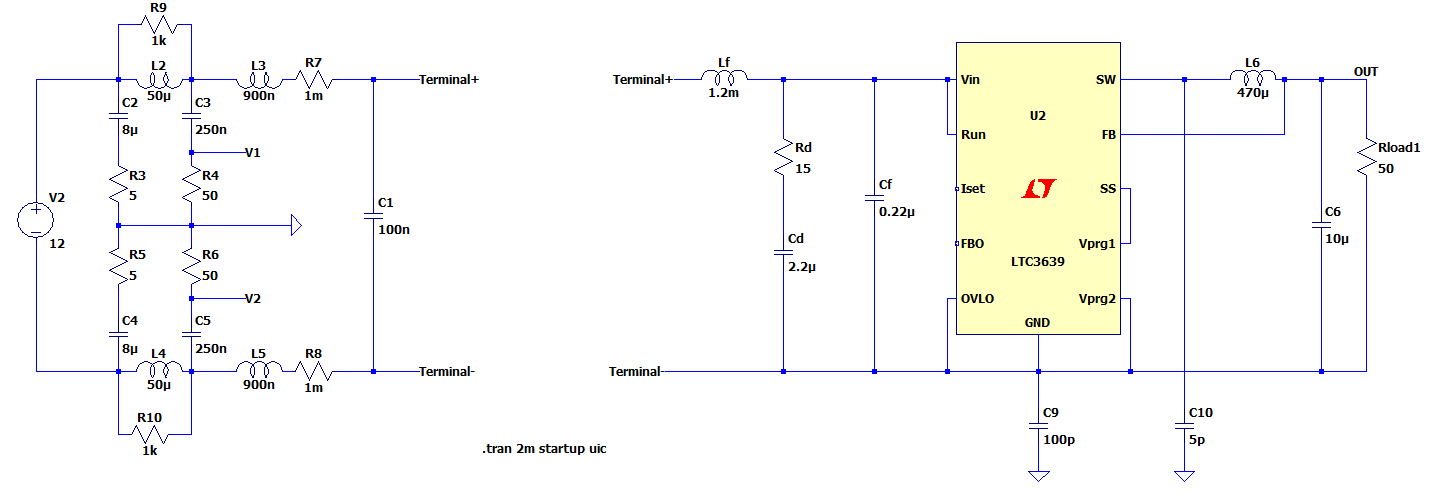
\includegraphics[width=0.8\linewidth]{Figure/LTC3639MitFilter.png}
    \caption{LTC3639 mit Filter}
    \label{fig:LTC3639MitFilter}
\end{figure}


\subsection{FFT}

In Abbildung \ref{fig:LTC3639MitFilterFFT} ist der FFT-Plot der Schaltung mit integriertem Filter dargestellt. Es ist erkennbar, dass der Filter seine Funktion erfüllt, indem er sowohl die Common-Mode- als auch die Differential-Mode-Störungen wirksam reduziert und unter die zulässigen Grenzwerte für die EMV-Zertifizierung verschiebt.


\begin{figure}[H]
    \centering
    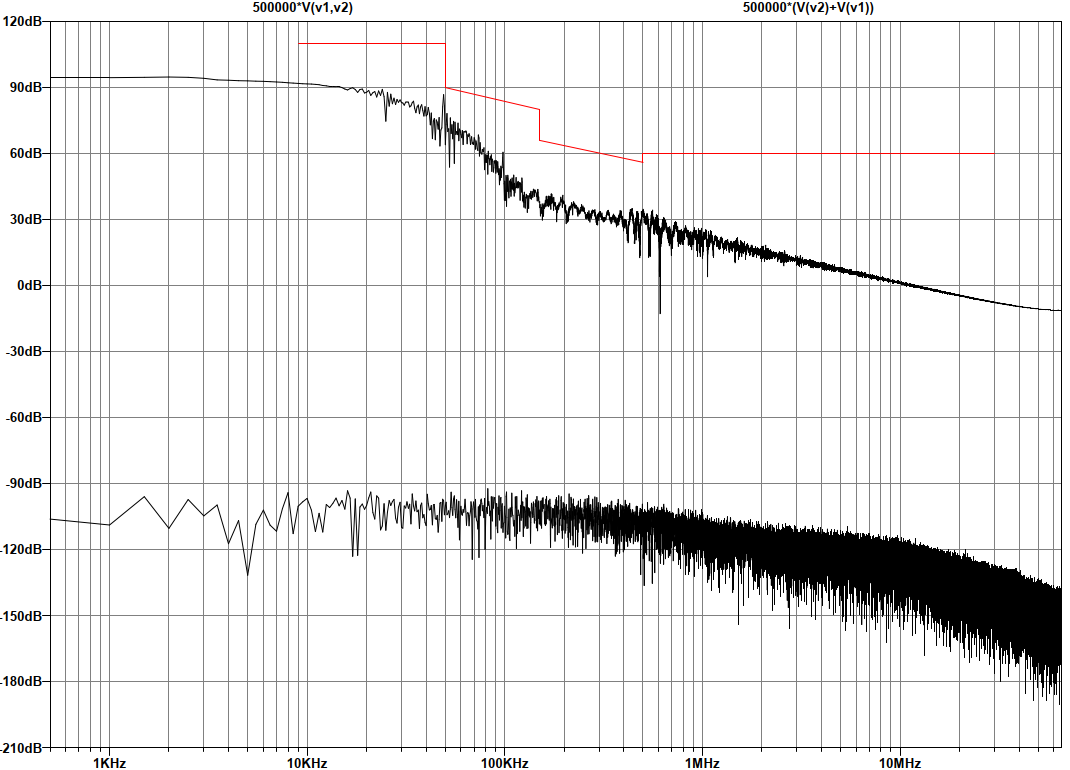
\includegraphics[width=0.8\linewidth]{Figure/LTC3639MitFilterFFT.png}
    \caption{FFT LTC3639 mit Filter}
    \label{fig:LTC3639MitFilterFFT}
\end{figure}